\documentclass[11pt,a4paper]{article}
\usepackage[T1]{fontenc}
\usepackage[utf8]{inputenc}
\usepackage{lmodern,microtype,amsmath,amssymb,amsthm,mathtools}
\usepackage{booktabs,longtable,array,enumitem,xcolor,geometry,fancyhdr,hyperref,graphicx}
\geometry{margin=21mm}
\hypersetup{colorlinks=true,linkcolor=blue!55!black,urlcolor=blue,
 pdftitle={FIN ST2172--ST2261: From Pair Kernels to Higher-Order Information},
 pdfauthor={Krzysztof Żuchowski}}
\pagestyle{fancy}\fancyhf{}
\fancyhead[L]{FIN ST2172--ST2261}\fancyhead[R]{Release 11.08}
\fancyfoot[C]{\thepage}\setlength{\headheight}{14pt}
\newtheorem{theorem}{Theorem}
\newtheorem{proposition}{Proposition}
\newcommand{\status}[1]{\textsf{[#1]}}

\begin{document}
\begin{titlepage}\centering\vspace*{13mm}
{\Huge\bfseries From Pair Kernels to Higher-Order Information\par}\vspace{4mm}
{\LARGE The Strict Loop-Product Flag Lift,\par}\vspace{2mm}
{\LARGE Hidden-Synergy No-Go and Adaptive Source Obstruction\par}\vspace{11mm}
{\Large FIN ST2172--ST2261\par}\vspace{8mm}
{\Large Krzysztof \.Zuchowski\par}
{\normalsize Independent Researcher --- Fractal Information Theory Project\par}
{\normalsize ORCID: 0009-0002-0909-3613\par}\vspace{8mm}
{\large Six adaptive research rounds --- 90 programmes\par}
{\large Release 11.08 --- 1 September 2026\par}
\vfill
\begin{minipage}{.88\textwidth}\small
This report tests the highest-value frontier left by Release 11.07: whether the
strict FIN pair kernel, its states, adaptive law, or fractal refinement can
source a mathematically unavoidable ternary/2-form object.  It identifies one
previously underclassified positive result---the strict loop-product flag
lift---and immediately subjects it to symmetry, probabilistic, adaptive,
refinement, Hodge-spectral, kernel-split and axiom-removal falsification.
\end{minipage}\vfill
{\small English mathematical research report. CC BY 4.0.}
\end{titlepage}

\begin{abstract}
Let \(A=sI-W\) be the strict twelve-state Dirichlet generator, with positive
off-diagonal conductances \(W_{ij}\).  Strict pair data generate a canonical
reducible three-cycle statistic
\[
 \tau_{ijk}=W_{ij}W_{jk}W_{ki}.
\]
All 220 triangle values are positive, lie in twelve \(D_{12}\)-orbits and
define a target-free weighted flag-complex candidate.  This corrects the
coarser earlier statement that the pair kernel generated no intrinsic
three-cycle observable.

The correction does not close the physical bridge.  The statistic \(\tau\) is
fully reducible to pair data and reflection-even.  A centered Gaussian theory
generated by a quadratic FIN action has vanishing connected third cumulants.
The functional-calculus algebra \(C^*(A)\) is commutative and associative.
State-dependent chiral currents exist, but the \(k=\pm1\) branches have equal
energy, opposite current and are exchanged by reflection.  Invariant mixtures,
\(D_{12}\)-twirls and Gibbs states have zero current.

The adaptive law \(\dot K=\Pi[C-V'(K)]\) does not repair the source problem
without additional data.  Spectral-algebra flows cannot generate a
noncommuting or odd structure.  Self-generated dephased covariance commutes
with \(A\), while its origin comes from preparation.  The strict \(W\) is
indefinite, so it cannot equal a positive covariance divided by positive decay
in the elementary linear Hebb fixed-point equation.

An exact information-theoretic obstruction is established using
\[
 p_\varepsilon(x_1,x_2,x_3)
 =\frac18(1+\varepsilon x_1x_2x_3),\qquad |\varepsilon|\leq1.
\]
Every member has the same complete one- and two-point records, while
\(\mathbb E[x_1x_2x_3]=\varepsilon\).  Marginalization erases the distinction.
No deterministic reconstruction from pair/coarse data can therefore recover
general irreducible ternary information.

The positive loop field yields an executable Hodge family
\[
 h_f(p)=\frac{\tau_f^p}{\langle\tau^p\rangle},\qquad p>0.
\]
Every member is positive, target-free and \(D_{12}\)-natural.  The choices
\(p=1\) and \(p=2\) give different one-form spectra with the same cohomology.
Current strict data therefore do not select unique gauge dynamics.

The smallest conditional uniqueness theorem needs four extra axioms:
triangle-edge locality, support-zero behaviour, separate linearity in each
edge coupling, and one universal face rule.  They imply
\(F(a,b,c)=\kappa abc\).  Removing any one admits explicit counterfamilies;
explicit permutation symmetry is redundant.  None of the four is yet derived
as a physical law.

The updated gate passes three strict mathematical rows and zero
physical-source rows.  FIN gains a rigorous higher-order graph lift, not a
sourced 2-form physical theory.  The next decisive theorem is to derive or
refute separate linearity and face universality from the strict
composition/refinement law.
\end{abstract}

\tableofcontents\newpage

\section{Scope and kernel discipline}

The legacy and strict objects remain separated:
\[
\begin{aligned}
K_{\rm legacy,ont}(d)
 &=\alpha_{\rm geo}\frac{\cos(\omega d+\phi)}{1+\beta_{\rm tors}d},\\
K_{\rm strict,gate}(d)
 &=\frac{\cos(\omega d+\phi)}{1+\beta d^\eta}.
\end{aligned}
\]
No legacy physical role is transferred.  The strict Dirichlet representation
used here is
\[
 A=sI-W,\qquad
 \langle f,Af\rangle
 =\frac12\sum_{x,y}W_{xy}|f_x-f_y|^2\geq0.
\]

Release 11.07 conflated two meanings that must be separated:
\begin{enumerate}[label=(\roman*)]
\item a three-cycle statistic derived from pair data;
\item irreducible third-order information not determined by pair data.
\end{enumerate}
The first exists.  The second is not generated by the current pair core.

\section{Round I: ST2172--ST2186 --- third-order classification}

The frozen strict matrix is invariant under all 24 elements of \(D_{12}\);
the finite conjugation residual is zero.

\begin{theorem}[fixed-input odd-scalar no-go]
If \(rx=x\) for a reflection \(r\), and \(F(rx)=-F(x)\), then \(F(x)=0\).
\end{theorem}
\begin{proof}
\(F(x)=F(rx)=-F(x)\).
\end{proof}

This applies to a global pseudoscalar derived equivariantly from the fixed pair
kernel.  It does not exclude oriented cochain bases or state-dependent odd
receivers.

For a centered Gaussian field, Wick's theorem gives
\[
 \langle\phi_i\phi_j\phi_k\rangle_c=0.
\]
Linear unitary, wave and heat evolution preserve Gaussianity.  Thus the dual
dynamics
\[
 U_t=e^{-itA},\qquad P_t=e^{-tA}
\]
do not create connected third cumulants from Gaussian data.

All Borel functions of one self-adjoint \(A\) commute, and matrix multiplication
is associative:
\[
 [f(A),g(A)]=0,\qquad
 (f(A)g(A))h(A)-f(A)(g(A)h(A))=0.
\]
The polynomial replay residuals were \(2.73\times10^{-13}\) and
\(4.23\times10^{-14}\); the exact facts follow from functional calculus.

\begin{proposition}[strict loop-product field]
\[
 \tau_{ijk}=W_{ij}W_{jk}W_{ki}
\]
is positive on all 220 strict triangles:
\[
 9.2543082\times10^{-5}\leq\tau_{ijk}
 \leq4.2419834\times10^{-2}.
\]
Its support values form exactly twelve \(D_{12}\)-orbits.
\end{proposition}

This is a local closed-walk statistic.  It is intrinsic as a graph observable
but is reducible to \((W_{ij},W_{jk},W_{ki})\), reflection-even, and not a
connected third cumulant.

\section{Round II: ST2187--ST2201 --- state chirality}

Let
\[
 \psi_k(n)=12^{-1/2}e^{2\pi i kn/12},\qquad
 \rho_k=|\psi_k\rangle\langle\psi_k|.
\]
For \(k=\pm1\),
\[
 \langle\psi_{\pm1},A\psi_{\pm1}\rangle=0.75412115420708.
\]
The state-kernel current
\[
 \Lambda(\rho,W)
 =\sum_i2\,\operatorname{Im}(\rho_{i,i+1}W_{i+1,i})
\]
gives
\[
 \Lambda(\rho_{+1},W)=-0.4699856726450202,\qquad
 \Lambda(\rho_{-1},W)=+0.4699856726450202.
\]
Reflection exchanges the two states with residual \(8.42\times10^{-16}\).

\begin{theorem}[invariant-state persistence]
If \(\Phi\) is \(D_{12}\)-covariant and \(\rho\) is \(D_{12}\)-invariant, then
\(\Phi(\rho)\) is invariant; every reflection-odd expectation remains zero.
\end{theorem}

The branch mixture has zero current.  The full twirl gives
\(-3.26\times10^{-18}\), and the Gibbs state gives zero.  The pitchfork
\(\dot q=(1-q^2)q\) has stable branches \(q=\pm1\) but does not select one.
Symmetric noise gives equal branch probabilities; a bias imports the missing
odd premise.

The P2718 chiral bispectrum and P3048 memory-phase triangle area remain real
odd receivers.  P3048 has five nonzero signed rows but zero accepted strict
source rows.  Chirality exists at state/receiver level, not as a selected
strict source.

\section{Round III: ST2202--ST2216 --- adaptive source audit}

The family
\[
 \dot K=\Pi[C-V'(K)]
\]
becomes a law only after \(C,V,\Pi\), initial state and time scale are supplied.

\begin{theorem}[commuting adaptive manifold]
If \(C(K),V'(K)\in C^*(K)\) and \(\Pi\) preserves this algebra, the flow remains
in \(C^*(K)\).  It cannot generate a noncommuting associator or odd source.
\end{theorem}

The dephased covariance of self-generated unitary motion is block diagonal in
the spectral projections of \(A\).  For a localized preparation it has rank
seven and
\[
 \|[A,C]\|_\infty=3.36\times10^{-16}.
\]
Translating the prepared delta changes it by Frobenius distance \(0.40824829\);
the apparent origin is preparation data.

For
\[
 \dot W=\eta(C-\gamma W),\qquad\gamma>0,
\]
the only fixed point is \(W=C/\gamma\).  Covariance is positive semidefinite,
whereas the strict \(W\) has
\[
 \lambda_{\min}(W)=-0.6818747624,\qquad
 \lambda_{\max}(W)=1.6603072788.
\]
The elementary covariance-Hebb law therefore cannot learn strict \(W\) as its
fixed point.  This is not a no-go for all nonlinear laws.  Reverse-engineering
\(V\) can make a chosen \(K\) stationary, but infinitely many potentials do
so; representation is not derivation.

\section{Round IV: ST2217--ST2231 --- exact hidden synergy}

\begin{theorem}[pair-sufficiency obstruction]
For
\[
 p_\varepsilon(x_1,x_2,x_3)
 =\frac18(1+\varepsilon x_1x_2x_3),\quad|\varepsilon|\leq1,
\]
one has
\[
 \mathbb E[x_i]=0,\quad
 \mathbb E[x_ix_j]=0\ (i\neq j),\quad
 \mathbb E[x_1x_2x_3]=\varepsilon.
\]
No deterministic function of the complete one- and two-point record can
recover the general third moment.
\end{theorem}
\begin{proof}
The binary-cube monomials are orthogonal characters.  All pair records are
identical, while the required output varies continuously.
\end{proof}

For \(\varepsilon=\pm0.75\), fine total-variation distance is \(0.75\).
Marginalizing any variable makes the pair distributions identical and the
distance zero.  Marginalization is coassociative, so order cannot recover the
erased synergy.

Conditionally, this formalizes the internal-layer intuition: a fine state can
carry ternary synergy invisible to a pair-limited coarse observer.  It does
not derive a physical observer or actual FIN probability law.

\section{Round V: ST2232--ST2246 --- flag-Hodge candidate}

All 66 strict conductances are positive; the minimum is \(0.0110708173\).
The support graph is \(K_{12}\), whose clique complex is the full 11-simplex
with 220 triangles.

Set
\[
 h_f(1)=\frac{\tau_f}{\langle\tau\rangle},\qquad
 L_1(h)=d_0d_0^*+d_1^*\operatorname{diag}(h)d_1.
\]
The \(p=1\) candidate has 33 distinct eigenvalues at eight decimal places and
\[
 0.3480858052\leq\lambda\leq60.2493296805.
\]

\begin{theorem}[positive-power Hodge counterfamily]
For every \(p>0\),
\[
 h_f(p)=\frac{\tau_f^p}{\langle\tau^p\rangle}
\]
is positive, target-free, \(D_{12}\)-natural, and has the same flag support.
All members have \(H^1=0\), but their positive spectra vary.
\end{theorem}

For \(p=1,2\),
\[
 \|\lambda(1)-\lambda(2)\|_\infty=24.78961896,
\]
with relative \(\ell^2\) distance \(0.3484\).  Mean-one normalization leaves
the trace equal.  Continuous positive multiplicative valuations have
\(g(x)=x^p\); refinement multiplicativity reduces the family but does not
select \(p\).  Setting \(p=\eta=1.8\) would be an unproved transfer from kernel
damping to face measure.

The complete support graph has diameter one and supplies no local wavevector,
lattice spacing, Lorentz cone or Maxwell limit.

\begin{figure}[ht]
\centering
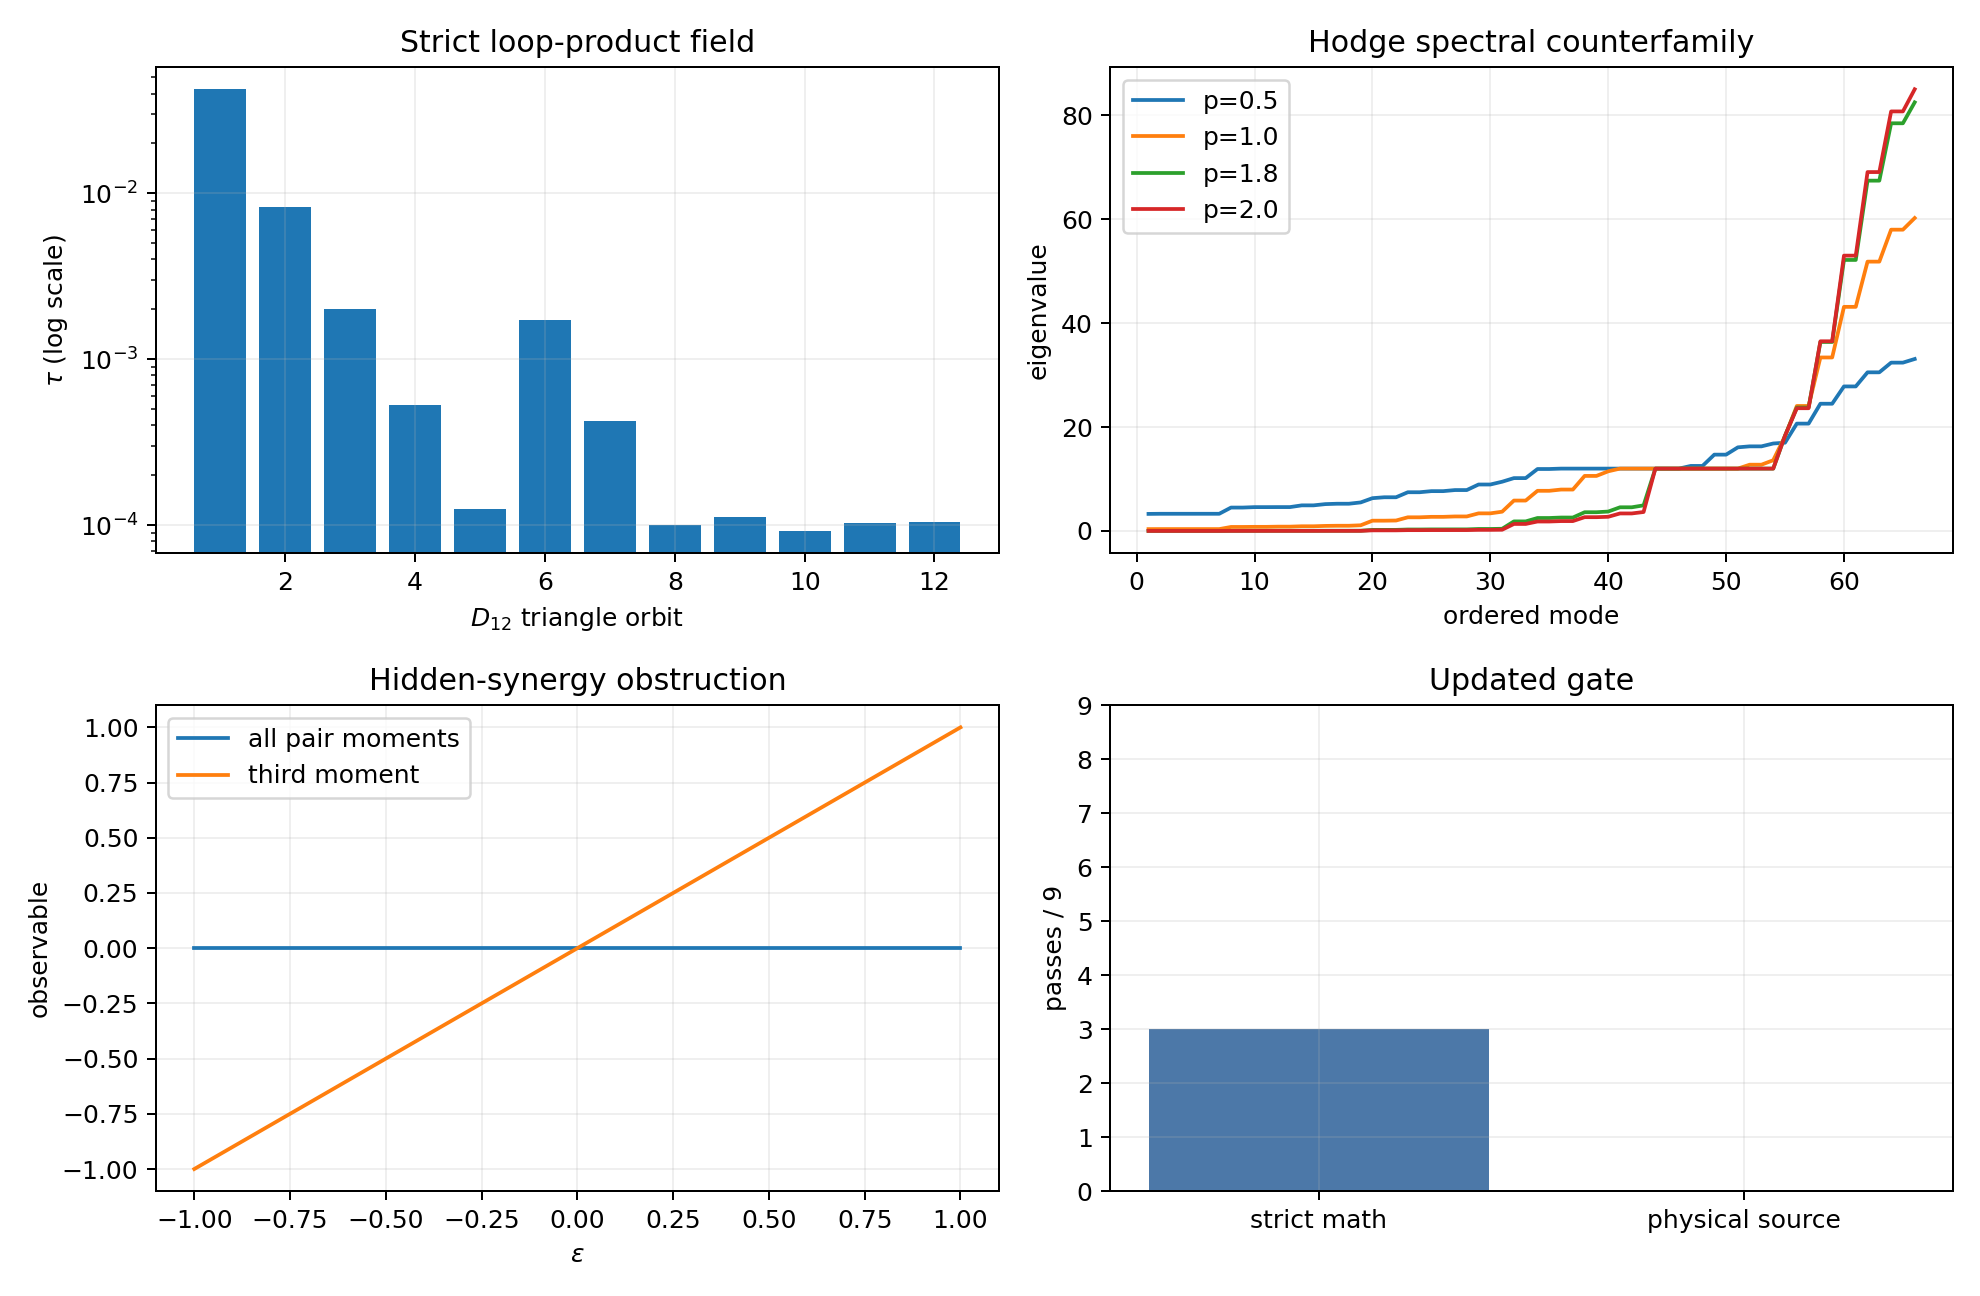
\includegraphics[width=.97\textwidth]{FIN_ST2172_ST2261_Figures/ternary_source_and_flag_hodge_audit.png}
\caption{Loop-product orbits; the Hodge spectral counterfamily; hidden
third-order synergy; and the updated mathematical-versus-physical gate.}
\end{figure}

\section{Round VI: ST2247--ST2261 --- minimal theorem}

Define the \emph{strict loop-product flag lift}
\[
 W\longmapsto
 \bigl(\operatorname{Clique}(\operatorname{supp}W),
       \tau_{ijk}=W_{ij}W_{jk}W_{ki}\bigr).
\]

\begin{theorem}[conditional uniqueness]
Suppose a face rule \(F(a,b,c)\) has:
\begin{enumerate}[label=\textnormal{\bfseries A\arabic*.}]
\item triangle-edge locality;
\item \(F=0\) if any support edge is absent;
\item separate linearity in each edge coupling;
\item one universal rule on every face, rather than one coefficient per
      \(D_{12}\)-orbit.
\end{enumerate}
Then \(F(a,b,c)=\kappa abc\).  Mean normalization fixes descriptive
\(\kappa\).
\end{theorem}

\begin{longtable}{@{}p{.12\textwidth}p{.22\textwidth}p{.52\textwidth}@{}}
\toprule
Axiom & Necessity & Result of removal \\
\midrule\endhead
A1 locality & necessary & arbitrary global invariant multipliers enter \\
A2 support-zero & necessary & constant, linear and pair terms enter \\
A3 separate linearity & necessary & \((abc)^p\) and general functions enter \\
A4 universality & necessary & twelve orbit coefficients enter \\
explicit symmetry & redundant & \(\kappa abc\) is already symmetric \\
\bottomrule
\end{longtable}

These axioms give a small conditional theorem.  A3 and A4 have not been
derived from strict dynamics or refinement.

\section{Updated gate and kernel-split falsification}

\begin{longtable}{@{}p{.45\textwidth}p{.18\textwidth}p{.20\textwidth}@{}}
\toprule
Requirement & Strict mathematics & Physical source \\
\midrule\endhead
reducible three-cycle observable & pass & fail \\
\(D_{12}\) law and nonzero witness & pass & fail \\
support-clique face complex & pass & fail \\
irreducible connected ternary source & fail & fail \\
nonpremise odd polarity & fail & fail \\
unique positive Hodge law & fail & fail \\
unique \(12\to24\to48\) ternary lift & fail & fail \\
dimensional local continuum scaling & fail & fail \\
OA platform and independent record & fail & fail \\
\bottomrule
\end{longtable}

\[
 \boxed{3/9\ \text{strict mathematical rows},\qquad
        0/9\ \text{physical-source rows}.}
\]

Strict positivity does not transfer to legacy.  Raw legacy triangle products
range from \(-12.3069\) to \(8.84166\), with 108 positive and 112 negative
faces.  A legacy positive Hodge model requires an additional absolute value,
square, sign sector or completion choice.  No bridge or legacy role transfer
follows.

\section{Result ledger}

\begin{longtable}{@{}p{.48\textwidth}p{.23\textwidth}p{.18\textwidth}@{}}
\toprule
Statement & Status & Scope \\
\midrule\endhead
strict positive three-cycle field & \status{Proven} & reducible statistic \\
Gaussian core generates third cumulant & \status{Refuted} & centered/linear \\
\(C^*(A)\) supplies associator & \status{Refuted} & one generator \\
chiral state current & \status{Proven} & prepared receiver \\
operator selects one chiral branch & \status{Refuted} & symmetric core \\
linear covariance Hebb learns strict \(W\) & \status{Refuted} & positive decay \\
pair data reconstruct ternary synergy & \status{Impossible} & exact theorem \\
weighted flag-Hodge model & \status{Constructed} & dimensionless \\
one strict Hodge law is selected & \status{Refuted} & power family \\
four axioms select \(\tau\) & \status{Conditional} & A1--A4 \\
continuum gauge physics & \status{Not established} & scale/OA absent \\
\bottomrule
\end{longtable}

\section{Deepest surviving interpretation}

\begin{quote}
The unavoidable higher-order shadow of the current strict FIN kernel is a
reducible loop-product lift of a weighted graph into its flag complex.  It is
not an irreducible three-point information law.  The operator supports
conditional discrete Hodge/gauge models but does not select their valuation
exponent, orientation sector, refined lift, physical units, continuum limit
or operational realization.  FIN remains a finite
Dirichlet--Markov--spectral information geometry with a newly explicit
higher-order graph lift, not a closed fundamental physical theory.
\end{quote}

\section{Next decisive programmes}

The highest-value next theorem is to derive or refute A3 and A4 from the
already strict composition/adaptive/refinement law, without importing the loop
product or \(p=1\).

Recommended ST2262--ST2276:
\begin{enumerate}[label=\textbf{ST\arabic*}, start=2262]
\item classify strict composition laws implying separate edge linearity;
\item test whether strict symmetry can force face universality;
\item classify continuous refinement valuations and exponent freedom;
\item audit edge-subdivision consistency of \(\tau\);
\item compute \(12\to24\to48\) loop-product renormalization;
\item construct a minimal hidden-synergy instrument;
\item test a sourced non-Gaussian adaptive third cumulant;
\item classify third cumulants under reflection-equivariant noise;
\item test strict selection of one chiral Fourier branch;
\item prove identifiability or nonidentifiability of \(p\);
\item test parameter-free sparsification without a threshold;
\item build a sign-safe legacy loop lift and list its extra axiom;
\item test one typed completion atom on triangle products;
\item write a conditional CA+SA+OA record model;
\item update the gate and stop if neither A3 nor A4 is derived.
\end{enumerate}

\section{Reproducibility and nonclaims}

Six result sets from
\texttt{FIN\_ST2172\_ST2186\_Results.json} through
\texttt{FIN\_ST2247\_ST2261\_Results.json} contain ninety packet hashes.
\texttt{test\_fin\_st2172\_st2261.py} verifies all hashes, cycle statistics,
state degeneracy, adaptive no-go, hidden synergy, Hodge counterfamily, gate and
figure.

This report does not derive an irreducible ternary state law, selector,
polarity, unique Hodge measure, physical scale, continuum gauge theory,
apparatus, record, legacy completion, legacy role transfer, \(QW\)-2191,
Standard Model, gravity, \(L_{\rm total}\), or Theory of Everything.

\begin{thebibliography}{9}
\bibitem{isserlis} L. Isserlis, On a formula for the product-moment
coefficient of any order of a normal frequency distribution,
\emph{Biometrika} \textbf{12} (1918), 134--139.
\bibitem{hatcher} A. Hatcher, \emph{Algebraic Topology}, Cambridge University
Press, 2002.
\bibitem{dec} M. Desbrun, E. Kanso, Y. Tong, Discrete Differential Forms for
Computational Modeling, in \emph{Discrete Differential Geometry},
Birkh\"auser, 2008.
\bibitem{repo} FIN local evidence packets and guardrails, Releases
11.03--11.08.
\end{thebibliography}
\end{document}
